% Chapter 1

\chapter{Discussion and Conclusion} % Main chapter title

\label{Chapter6} % For referencing the chapter elsewhere, use \ref{Chapter1}

\lhead{Chapter 6. \emph{Discussion and Conclusion}} % This is for the header on each page - perhaps a shortened title

%----------------------------------------------------------------------------------------

In this section the planning for robots to accomplish the common objective is discussed in this work. To solve the problem of robots concurrent activities in an environment by avoiding hurdles many algorithms are available but solving the problem by using these techniques may increase the complexity of the solution which is difficult to implement. Temporal Logics may reduce the complexity and the formal techniques make easier to implement.
\section{Outcomes after verification}
To solve these problems for multiple robots that they can perform concurrent activities many algorithms are available but solving the problem by using these algorithms increases the complexity of the solution which becomes difficult to implement.

We implement different processes in spin and after that the results are verified. Outcomes are depend on the verification of the process. When program is executed then we check its safety and liveness properties then we get the result which is shown in figure 6.1 and figure 6.2:

\begin{landscape}
\begin{figure}[h]
\centering
  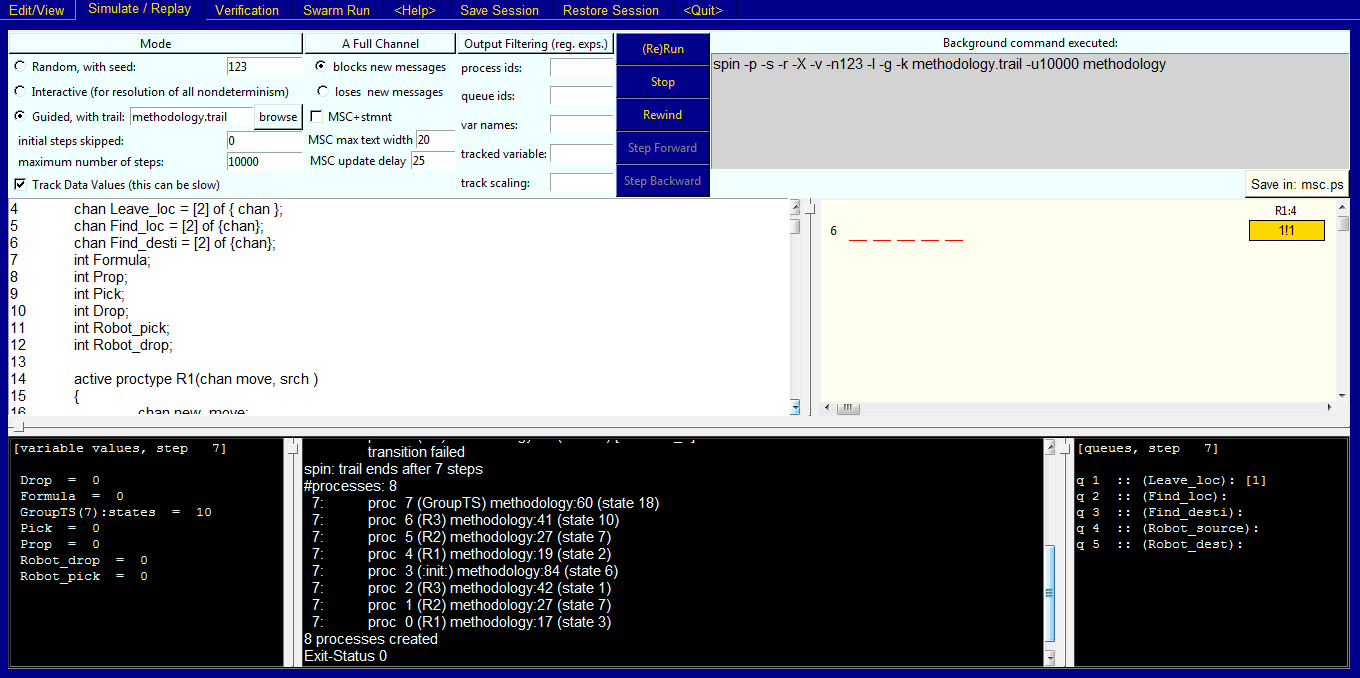
\includegraphics[width=19cm, height=13cm]{k}\\
  \caption{Result after simulation}
\end{figure}
\end{landscape}

\begin{landscape}
\begin{figure}[h]
\centering
  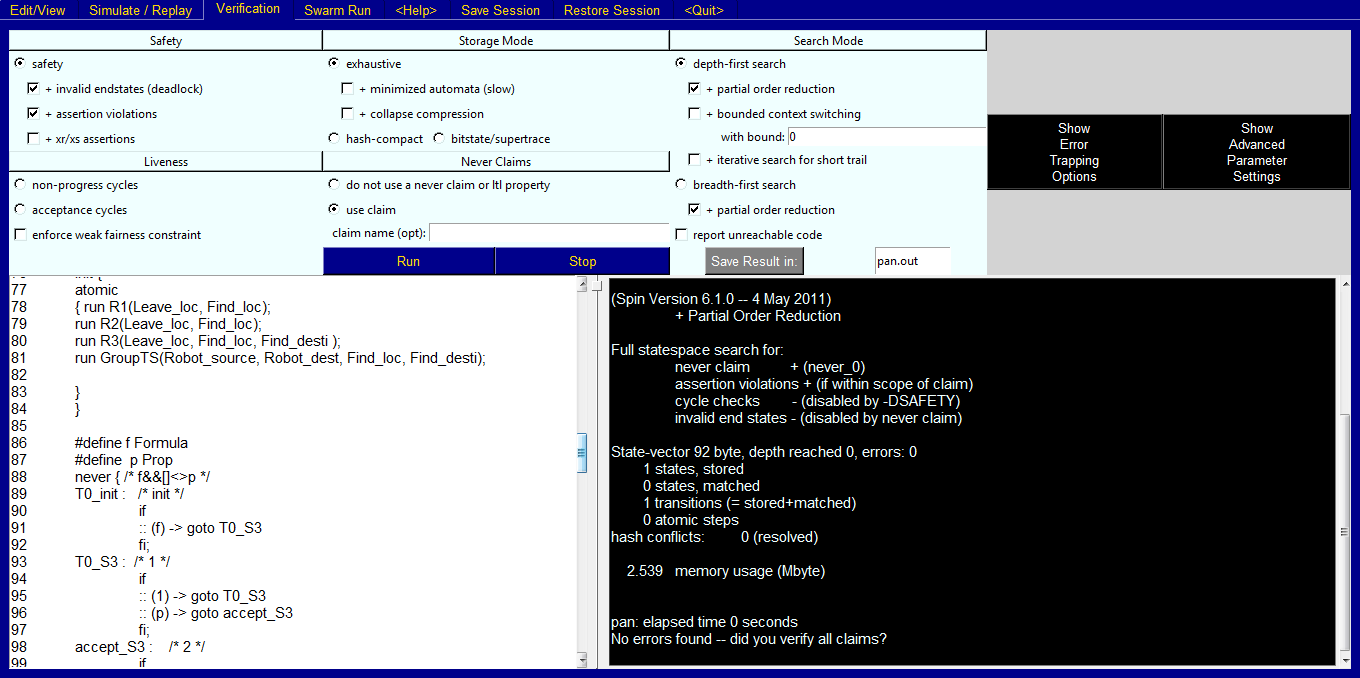
\includegraphics[width=19cm, height=13cm]{l}\\
  \caption{Result after verification}
\end{figure}
\end{landscape}

\pagebreak
\section{Conclusion}
A sample Conclusion 
A method is presented in this work for modeling the concurrent activities of a group of robots using temporal logics. The specifications are expressed in LTL formula and an algorithm is provided to model the transition system for the group of robots. Our method is optimal in a computational way as compared to previous methods, in which they constructed a model that captures all group members and their mission specification. The main drawback is the complexity of previous models that are time consuming processes.

Our approach is optimal to handle such cases where robots can take an action after confirmation of path availability according to the plan, and in some applications they has practical value where a series of different tasks performed by multiple robots in an environment. For some applications including new states and corresponding transitions to the structure of the robotic system may indicate to introducing advance stages or motion commands at some lower level. So the proper way in which the changes of these models are strictly application specific and we do not consider such details in our work. Assuming that these changes can be implemented in future........


